\clearpage
\section{Method}
\label{sec:method}

Our method consists of three parts.
Initially, we establish a metric based on the concept of the 15-minute city and extend it with cost.
Following this, we focus on finding a fitting routing algorithm to calculate this metric.
We do so by clearly stating our requirements for such an algorithm, explaining why existing algorithms don't meet our criteria, and introducing our algorithm, designed to meet our needs. 
The final stage explains how we use our routing algorithm to calculate our metric. 
This approach allows us to analyze accessibility in urban settings, offering valuable insights for urban planners and decision-makers.

\subsection{Metric}
\label{subsec:metric}

Our metric is based on the concept of the 15-minute city and expands on the findings of \shortciteA{olivariAreItalianCities2023}.
It consists of two dimensions: time and cost.
The time dimension effectively measures how fast the access to various essential amenities is, and the cost dimension measures how expensive this access is.
To measure this, we categorize amenities into seven essential services: grocery, education, health, banks, parks, sustenance, and shops.
Each category is populated with Points of Interest (POIs) sourced from OSM, providing a comprehensive database of locations.
The POIs are identified by their respective OSM tags.
OSM tags are descriptive labels used to define the attributes and characteristics of geographic features in the OSM database. 
They consist of a key and a value pair, like "amenity=restaurant", which enables categorizing map elements such as roads, buildings, and natural features for accurate and comprehensive mapping.
In our case, we use the OSM tags to identify nodes that represent POIs, like a supermarket or a park.
The categories and their respective tags can be seen in Appendix \ref{app:categories_and_osm_tags}.

The core of our metric is the determination of temporal proximity to these amenities. 
For each category, we calculate the minimum travel time required to reach at least one POI of that category. 
The metric is then defined as the maximum value among these minimal times across all categories.
We refer to it as the X-minute city metric, where X represents the maximum value among the minimum travel times.
This approach yields a singular measure that reflects the least accessible category for any given region.
We think that it is beneficial to focus on the least accessible category, as measuring accessibility in cities by averaging accessibility across all categories can mask disparities. 
Our approach ensures that the metric is targeted at areas of greatest need. 
In addition, our metric can directly reflect the original definition of a 15-minute city: if the X-minute city metric is below 15 minutes, the city can be considered a 15-minute city.
By leveraging this metric, we aim to help city planners create urban environments that prioritize sustainability, enhance the well-being of residents, and reduce dependency on motorized transport, thus contributing to the broader goals of efficient urban planning and improved quality of urban life.

% --- comparison to NEXI
Our metric presents several advantages compared to the NEXI-minutes and NEXI-global, as outlined by \shortciteA{olivariAreItalianCities2023}.
Firstly, unlike the NEXI-minutes, which calculates separate metrics for each of the seven categories, our metric evaluates all categories together. 
This unified approach is more straightforward to understand. 
In contrast, while NEXI-global considers all categories in one assessment, it converts the results into a 0-100 score. 
This scoring system can obscure the actual value of the data, making it more challenging to interpret.

Moreover, the NEXI-global's practice of assigning different weights to each category complicates its analysis. 
By focusing on the lowest-performing category across all areas, our metric simplifies the understanding and highlights where improvement is most needed. 

% --- cost
In addition to the time dimension, we incorporate a cost dimension into our metric.
As we want to incorporate more modes than just walking, some of which may have a monetary cost associated with them, we need to consider the cost of the trip.
We recognize that time and cost are measures of different units and cannot be combined sensibly.
Therefore, we draw upon Pareto optimality to create a multi-objective metric considering time and cost.
We define a Pareto set as a set of tuples where each tuple contains a time value and a cost value.
A tuple can be considered the time needed to reach all categories given the cost value.
The Pareto set will allow answering questions in the form of "What is the fastest time I can reach any categories given a certain cost?" or "What is the lowest price I need to pay to reach all categories given a certain time?".


\subsection{Routing Algorithm}
\label{subs:routing_algorithm}
Traditionally, the 15-minute city concept is applied to walking and cycling and ignores other modes of transport.
In the context of location-based metrics, some researchers even go as far as to only calculate the bee-line distance to the nearest amenity and ignore the street network altogether \shortcite{gastnerOptimalDesignSpatial2006}. At the same time, most only consider walking \shortcite{olivariAreItalianCities2023, nicolettiDisadvantagedCommunitiesHave2023}.
As explained in Section \ref{subsec:importance_of_multimodality_and_intermodality}, to determine the accessibility of a city accurately, we have to consider all modes of transport.
To do so, we require a routing algorithm that is capable of including multiple modes of transport, which we develop in this Section.
First, we define the requirements for our routing algorithm and explain why existing algorithms don't meet our criteria.
Next, we explain our algorithm in detail, which is based on a modular approach, where one module represents the usage of one mode of transport for a segment of the trip.
After that, we explain these modules, which are based on MLC or McRAPTOR.
Lastly, we explain some enhancements we made to MLC and McRAPTOR to support more dynamic multi-objective optimization.

\subsubsection{Requirements}
\label{subsubsec:requirements}

To fully grasp the potential of the combination of the sustainable modes of transport, we require our routing algorithm to be \textbf{multi-modal}, \textbf{multi-objective}, \textbf{unrestricted inter-modal}, and \textbf{modular}.

\textbf{Multi-modal} means that our routing algorithm allows multiple modes of transport, including scheduled transport systems, like public transport, and an arbitrary number of unscheduled transport systems, like walking, cycling, and driving.
In addition, we require that free-floating vehicle-sharing systems are incorporated realistically.
That means that our routing algorithm must consider that switching to a free-floating vehicle is possible at any location where a free-floating vehicle is available, and parking a free-floating vehicle is possible anywhere it is allowed.

\textbf{Multi-objective} means that our algorithm must find all Pareto optimal journeys according to an arbitrary amount of objectives.
The algorithm must provide the possibility to update the values of any objective whenever a movement occurs.
We define a movement as an edge traversal in an unscheduled network or a step in the route traversal in a scheduled network.
% In the case of an edge traversal, the new objective must be a function of the old objective and the edge weights, formally: \(l' = f(l, w(e))\), where \(l\) and \(l'\) are the old and new labels, respectively, and \(w(e)\) are the weights of the edge that is traversed.
% In the case of an update during a step of the route traversal, the new objective must be a function of the old objective (to be continued).

\textbf{Inter-modal} means the different transport modes may be sequenced in any order.
For example, when considering walking, cycling, and public transport, the algorithm must consider journeys with any combination of these modes in any order.

\textbf{Unrestricted} means that the algorithm thoroughly searches the unscheduled network graphs and does not pose restrictions like a maximum of 10 minutes walking distance.

\textbf{Modular} means that the algorithm should be easily adaptable to different modes of transport.
It should be possible to easily add, remove, or chain different modes of transport.


Next, we explain why the algorithm introduced in Section \ref{subsec:routing_algorithms} do not meet these requirements.
Both Dijkstra and MLC are not considered due to their impractical runtime.
Furthermore, the need for multi-objective solutions excludes Dijkstra, RAPTOR, and ULTRA.
The requirement for unrestricted inter-modal travel makes RAPTOR and McRAPTOR unsuitable in practical scenarios.
To explain this, let's examine a straightforward example.
Consider the OSM graph of the key regions in Cologne, which comprises 125,176 nodes and 142,074 edges.
For RAPTOR to compute a transitively closed graph requires calculating the walking distance between each node.
This computation would yield \(125,176^2 = 15,669,030,976\) edges, vastly greater than the original 142,074 edges.
While MCR does support multi-objective solutions with unrestricted inter-modal transfers, the transport modes it supports are limited.
Although it theoretically permits various modes of unscheduled transport, it is primarily tailored for station-based vehicle-sharing systems.
Our focus, however, is on the increasingly prevalent free-floating systems.
Moreover, unscheduled networks are contracted in MCR, leading to the removal of specific nodes.
If an optimal route requires a mode change at a deleted node, MCR will be unable to identify that path.
As a result, MCR is not a viable option for our requirements.
Also, note that none of the algorithms mentioned so far are modular, meaning the considered transport modes cannot be easily added or removed.
Without modularity, it is not possible to compare different combinations of transport modes, which is a crucial aspect of our work.

\subsubsection{Scaffolding Framework}
\label{subsubsec:algorithm}

% introduction modules
As mentioned above, our routing algorithm should be easily adaptable to different modes of transport. Therefore, we formulate it in a modular fashion as a scaffolding framework.
Next, we describe a scaffolding framework that needs to be augmented by different modules, where a module represents a single usage of a specific transport mode. Running a module can be seen as exploring the corresponding network through this mode of transport.
One module, for example, would be walking, and running the walking module would mean traversing the whole walking graph, given the current state of the bags.

% explanation of bags & need for common network 
A module always takes bags as an input and returns bags as an output.
As explained in Section \ref{sec:related_work}, a bag is a set of Pareto optimal labels attributing specific values to each objective.
In our work, a bag is additionally associated with a node on some network.
For the bags that are the input and output of the modules, we further require that they are associated with the common network.
This is necessary to feed the output bags of one module into the input bags of another module.
The most reasonable choice for the common network is the walking graph, which has a real-world interpretation because walking between different modes of transport is very common.

% example of running a module
To explain how a module is run, consider a set of starting bags that is used as input for the walking module.
In the starting bags, each bag is empty except for the starting node's bag, which contains one label with the start time and no costs.
The output would be a set of bags, where each node's bag contains exactly one label, where the time would be equal to the time it takes to walk to the node, and the cost would be zero, as walking never costs anything.

% algorithm
The scaffolding framework is shown in Figure \ref{fig:modular_routing_algorithm}.
It is configured by two module matrices, the initial module matrix and the repeating module matrix, and the maximum number of transfers.
A module matrix is an irregular matrix where each entry is a module.
The matrix specifies the order in which modules are run and whether they are run sequentially or in parallel.

Running the framework begins with a start node and time as input.
Its output is a set of bags.
It first creates the starting bags described above from the start node and the start time.
Next, it runs the initial modules given by the initial module matrix.
To run a module matrix, the first row's modules are run in parallel.
Their respective outputs are then merged into a single set of bags, which is used as the input for the second row's modules.
This process repeats for each row of the module matrix.
After the initial module matrix is run, the same is done for the repeating module matrix.
The repeating module matrix, in comparison to the initial module matrix, is run multiple times, as often as the specified maximum number of transfers.
By convention, we count each iteration of the repeating modules as one trip.

\begin{figure}
    \centering
    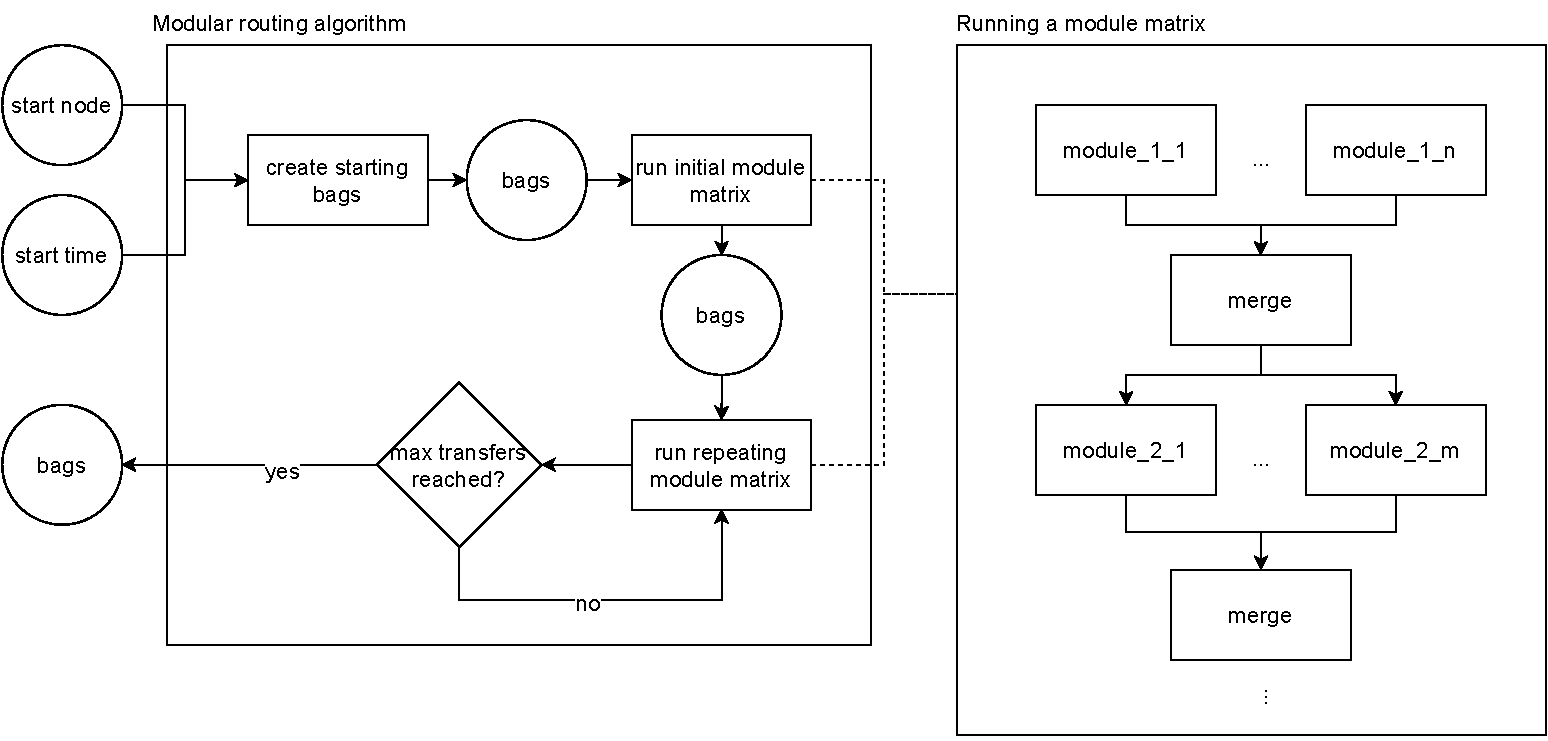
\includegraphics[scale=0.40]{Figures/method/modular_routing_algorithm}
    \caption{Scaffolding Framework}
    \label{fig:modular_routing_algorithm}
\end{figure}


\subsubsection{Modules}
\label{subsubsec:modules}

In our experiments, we categorize our modules into two types: unscheduled and scheduled. 
The unscheduled modules consist of walking, free-floating bicycle sharing, and personal vehicle use, which are based on MLC. Meanwhile, the scheduled module is public transport, which is based on McRAPTOR.

Walking is the most straightforward unscheduled module, which consists of running MLC on the walking graph.
The edges of the walking graph should contain the time it takes to traverse them by foot and should not have any monetary cost associated with them.

The free-floating bicycle-sharing module is more complex than the walking module.
Before running MLC on the respective bicycle graph, the module filters all bags located at a node where no free-floating vehicle is available, as it is only possible to start a trip with a bicycle from nodes where a bicycle is present.
In addition, the vehicle graph is augmented with a walking graph. 
This means that at nodes in the vehicle graph where the vehicle is allowed to be parked, there is an edge to the closest node in the walking graph.
This augmentation is necessary, as the output bags of the free-floating vehicle-sharing module must be associated with nodes in the walking graph, as it is the common network.
The module can also define cost depending on the time spent on the trip.

For the personal vehicle module, we assume that there is only one personal vehicle and that it is located at the starting node.
Therefore, the module filters out all bags not located at the starting node.
Obviously, this module is intended to be used before any other module is used, i.e., for the first segment of the trip.
Therefore, it should only appear in the first row of the initial module matrix.
After that, MLC is run on the personal vehicle graph, augmented with the walking graph.
As this module is also based on MLC, it can define costs like the free-floating vehicle-sharing module.

Compared to the unscheduled modules, the public transport module does not use MLC but McRAPTOR.
As a first step, the module filters out all bags associated with nodes that are not near a stop in the public transport system.
Next, the module performs a single iteration of McRAPTOR, representing a single trip within the public transport system.
Finally, the resulting bags need to be re-associated with the nodes of the walking network.
To do so, the module uses the node closest to the coordinates of the public transport stop.
The public transport module can define costs like the free-floating vehicle sharing and personal vehicle modules.
The cost may depend on the number of stops traversed during the trip.

\subsubsection{Merging}
\label{subsubsec:merging}

The merging of bags after running multiple modules in parallel is quite simple.
Each bag represents a set of Pareto optimal labels, and each bag is associated with a node.
We, therefore, merge node-wise.
We differentiate between two cases:
\begin{enumerate}
    \item There is only one bag associated with a node.
    \item There are multiple bags associated with the same node.
\end{enumerate}
In the first case, we directly put the bag into the output bags.
In the second case, we create a new bag that contains all labels of all bags associated with the node, which might break the Pareto optimality of the labels.
Therefore, to restore the Pareto optimality of the labels, we remove all labels dominated by another label.

\subsubsection{Enhanced MLC \& McRAPTOR}
\label{subsubsec:enhanced_mlc_and_mcraptor}

To address the multi-objective optimization involving both time and monetary cost, we introduce enhancements to MLC and McRAPTOR. 
The standard versions of MLC and McRAPTOR do not adequately capture dynamic pricing models, which is necessary to represent monetary costs realistically.

The original MLC associates a fixed cost with an edge, which cannot represent variable pricing, such as a bike-sharing tariff that costs \euro{1} per 15-minute increment. 
Labels are only updated by adding the cost of a given edge to the label's values.
Similarly, McRAPTOR updates the labels at each stop during route traversal only based on the information of the current trip and stop. 
With this, McRAPTOR cannot represent a pricing scheme that changes in discrete steps depending on the number of stops, like the one used by the Cologne Transport Authority.
Our proposed modifications involve the use of hidden values within the labels that are used by these algorithms. 
These hidden values carry additional information that is not considered when comparing labels, but that may be used to update costs dynamically.

In the case of MLC, the hidden values may be updated along any edge, just like the regular values of the label.
A hidden value may carry information on how long the current trip with the shared vehicle is.
We also allow defining a function that updates while traversing an edge and may use the values and hidden values before and after the traversal to do the update.
With this functionality, it is easy to increment the cost by \euro{1} every time the time spent on the trip exceeds the 15-minute interval.

Similarly, the hidden values may be updated during McRAPTOR after every iteration of a stop.
We can, therefore, store how many stops the current trip has already traversed, and if that number exceeds four, we can increase the price from \euro{2.20} to \euro{3.20}.

Additionally, as the concept of hidden values isn't specific to MLC or McRAPTOR, the hidden values can be transferred across iterations and modules.
To understand the benefit, again consider the example of the pricing of the Cologne Transport Authority.
The ticket that costs \euro{3.20} allows traveling any number of trips within Cologne, no matter if changing to a different trip is necessary.
Therefore, if we were to first travel to two stops with one trip and then get out to catch another trip that consists of five stops, we would still have the information that we already commuted two stops.
Therefore, we can charge \euro{3.20} instead of \euro{2.20} twice, which is more realistic.
These enhanced versions of MLC and McRAPTOR are used in our modules to use more realistic dynamic pricing schemes.

While running our experiment, we found out that MLC-based modules present a significant computational bottleneck.
To calculate our metric, we don't need the labels of every single node but only those that impact the X-minute city and time Pareto front.
Therefore, we introduce a runtime optimization into MLC, which eliminates some bags from being processed that are guaranteed not to impact the Pareto front.
While iterating the unprocessed bags in MLC, we keep track of the minimum time required to reach a POI node of each category for each cost value.
If we encounter a bag whose time and cost values are greater than the minimum time and cost values for all categories, we can safely discard this bag, as it will not impact the Pareto front.


\subsubsection{Example}
\label{subsubsec:example}

To illustrate our algorithm, we go through an example.
The module configuration we use in our example represents traveling by free-floating vehicle sharing, public transport, and walking.
The initial module matrix contains the walking module to reach the free-floating vehicles and the public transport stops.
The repeating module matrix consists of first the free-floating vehicle sharing module and the public transport module in parallel and then the walking module.
It can be seen in Figure \ref{fig:example_module_matrix}.


\begin{figure}[ht]
\centering
\[
\begin{pmatrix}
\text{free-floating vehicle} & \text{public transport} \\
\text{sharing module} & \text{module} \\
\\
\text{walking module} & \\
\end{pmatrix}
\]
\caption{Example Repeating Module Matrix}
\label{fig:example_module_matrix}
\end{figure}

In our example, we assume that both public transport and vehicle sharing have some form of cost associated with them.
The objective is to minimize arrival time and cost.
We also consider a maximum of two trips.

First, we run the initial modules, which in our case is just the walking module on the starting bags.
As the starting bags only consist of one non-empty bag at the starting node with precisely one label, running MLC on the walking graph is equivalent to running Dijkstra's algorithm.
In the real world, this represents walking to all nodes in the walking network from the start node.
Note that after the initial walking module, all bags contain exactly one label, as the cost to go anywhere on foot is zero.

Next, the modules of the first row of the repeating matrix are run in parallel.
In the real world, this means that after an initial walk, the traveler would either drive with a free-floating vehicle starting from a location where one is available or commute by public transport starting from some stop.
The modules simultaneously compute all possible trips.
For the public transport module, for example, one could imagine commuting along all possible routes from all stops and updating the bags at the stops along each route accordingly.
After running these modules and merging their result bags, each bag may contain more than one label, as public transport and driving with a vehicle may be faster than walking but also cost money.
It may even be that some bags contain three different labels, if, for example, driving with a vehicle is the fastest but also costs the most money and commuting by public transport is faster than walking.
The next step consists of running the second row of the repeating module matrix, which, in our case, is the walking module again.
Running the walking module in the repeating module matrix is essential to reach nearby POIs after commuting through the public transport system.
After that, the repeating module matrix is rerun, as we consider a maximum of two trips.
The result of the second run of the repeating module matrix is our final result.

\subsection{Integrated Accessibility Analysis Routine}
\label{subsec:combining}

We embed the framework described in Section \ref{subsubsec:algorithm} in our accessibility analysis routine to compute the metric described in Section \ref{subsec:metric}.
Our accessibility analysis routine consists of three parts: the input routine, the main routine, and the metrics routine.

% Input routine
\begin{figure}
    \centering
    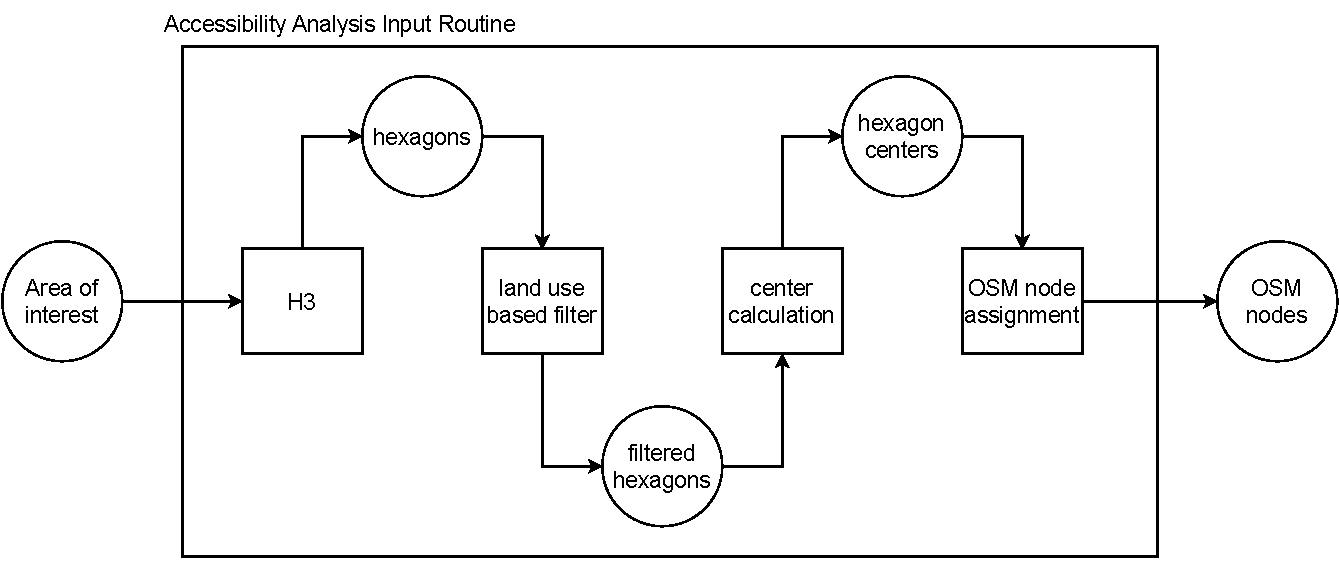
\includegraphics[scale=0.50]{Figures/method/input_routine}
    \caption{Input Routine}
    \label{fig:input_routine}
\end{figure}
In the input routine, depicted in Figure \ref{fig:input_routine}, we first create an even grid that covers the whole area of interest, for example, a city.
We use H3 \shortcite{H3H32023}, which uses hexagons to discretize an area to create such a grid evenly.
Our goal is to calculate our metric for each hexagon to get detailed spatial information about the accessibility in the area of interest.
Thus, selecting the right H3 resolution requires careful consideration of the tradeoff between finer detail and the impact on computation time.
We recommend a resolution of nine, corresponding to a hexagon edge length of roughly 200 meters, as it is a good compromise between accuracy and computation time when running the algorithm on consumer hardware. 
The input routine also filters out uninteresting hexagons.
For example, we filter out hexagons containing no residential areas, as no people are living there.
Next, the input routine retrieves the centroid of each hexagon and then calculates the Euclidean distance between the centroids and the OSM nodes to assign the closest OSM node to each centroid.
The result of the input routine is a set of OSM nodes for which we want to compute the accessibility.


% Main routine
\begin{figure}
    \centering
    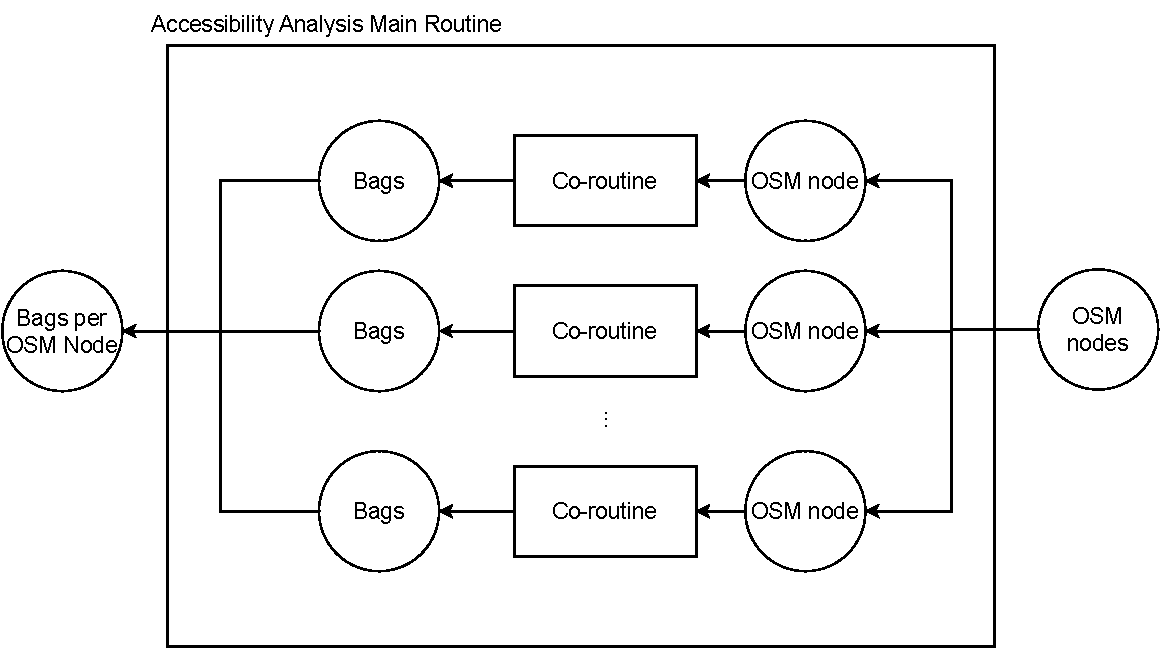
\includegraphics[scale=0.50]{Figures/method/main_routine}
    \caption{Main Routine}
    \label{fig:main_routine}
\end{figure}
The main routine, depicted in Figure \ref{fig:main_routine}, calls our scaffolding routing algorithm described in Section \ref{subsubsec:algorithm} on each OSM node provided by the input routine.
This results in a set of bags for each node.

% Metrics routine
\begin{figure}
    \centering
    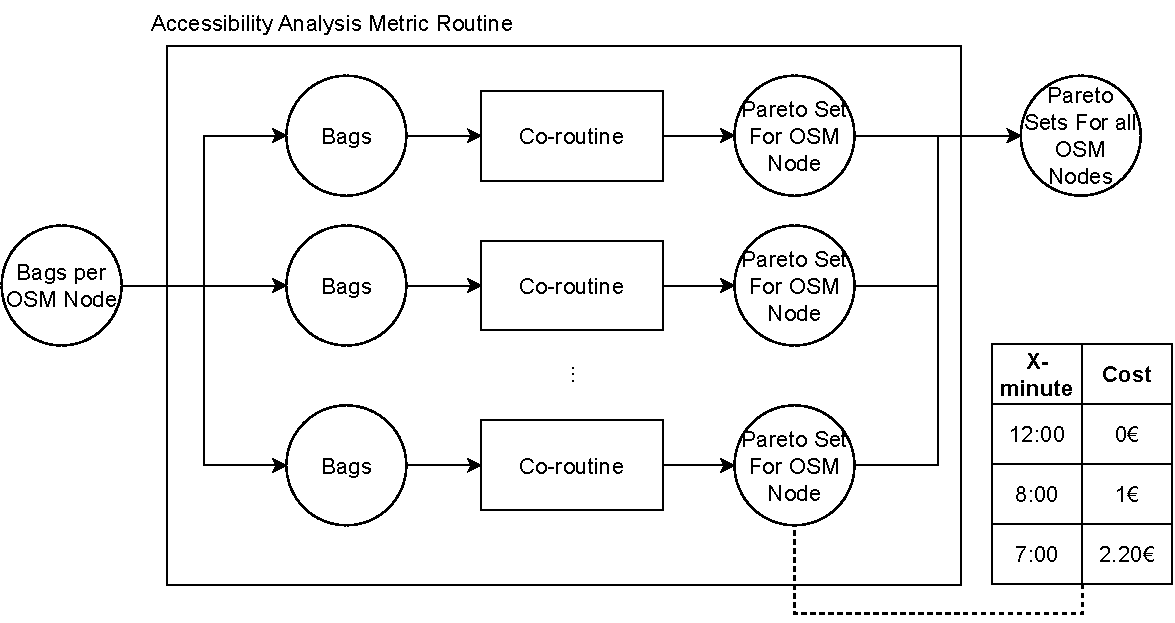
\includegraphics[scale=0.50]{Figures/method/metric_routine}
    \caption{Metric Routine}
    \label{fig:metric_routine}
\end{figure}
The metrics routine, depicted in Figure \ref{fig:metric_routine}, processes the bags into Pareto sets, where one entry in the Pareto set is a tuple of the X-minute city metric and the related cost.
To do so, we process each collection of bags separately - one co-routine for each OSM node/collection.
The co-routine is depicted in Figure \ref{fig:metric_co_routine} and works as follows.
We start by collecting all unique cost values on each label in each bag and then sorting them in ascending order.
For each cost value, we then determine the associated X-minute city metric.
We check whether every category is reachable given the cost value and an iteratively increasing time value.
We start with a time value equal to the minimum time across all labels.
If all categories are reachable, we've found the X-minute city metric, which, together with the cost value, is added to the Pareto set.
If not, we increase the time value by one minute and check again.
We repeat this until all cost values are processed.
The result is a Pareto set for each OSM node.

\begin{figure}
    \centering
    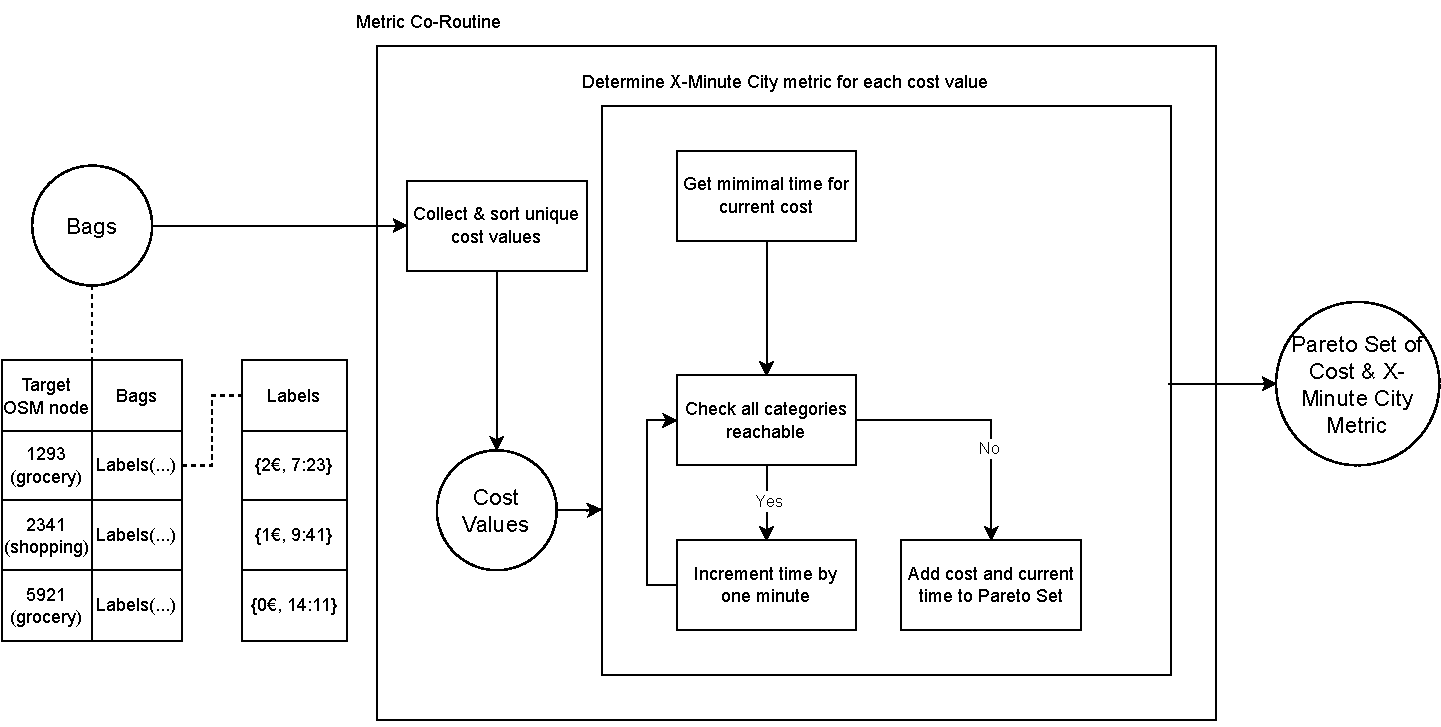
\includegraphics[scale=0.60]{Figures/method/metric_coroutine}
    \caption{Metric Co-Routine}
    \label{fig:metric_co_routine}
\end{figure}
